\documentclass[letterpaper,12pt]{article}
\usepackage{dgjournal}          
\usepackage{mathptmx}
\usepackage{graphicx} % Allows use of width and scale options for \includegraphics
\usepackage{hyperref} % To create hyperlinks in the paper
\usepackage[authoryear,comma,longnamesfirst,sectionbib]{natbib} 
%% The lineno packages adds line numbers. Start line numbering with
%% \begin{linenumbers}, end it with \end{linenumbers}. Or switch it on
%% for the whole article with \linenumbers after \end{frontmatter}.
\usepackage{lineno}
\linenumbers % Turns on line numbering for the entire document.

\begin{document}

%% Do NOT include any frontmatter information; including the title, author names,
%% institutes, acknowledgments and title footnotes (author information, funding
%% sources, etc.). Start the document with the first section or paragraph of
%% the article.

%%%%%%%%%%%%%%%%%%%%%%%%%%%%%%%
\section*{Abstract}
%%%%%%%%%%%%%%%%%%%%%%%%%%%%%%%


%%%%%%%%%%%%%%%%%%%%%%%%%%%%%%%
\section*{To Do Items}
%%%%%%%%%%%%%%%%%%%%%%%%%%%%%%%

\begin{itemize}
\item{Heun: Fix CDC reference to include volume and issue.} 

\end{itemize}




%%%%%%%%%%%%%%%%%%%%%%%%%%%%%%%
\section{Introduction}
\label{sec:introduction}
%%%%%%%%%%%%%%%%%%%%%%%%%%%%%%%


%%%%%%%%%%%%%%%%%%%%%%%%%%%%%%%
\section{Sources of data}
\label{sec:sources_of_data}
%%%%%%%%%%%%%%%%%%%%%%%%%%%%%%%

**** Caleb complete this section ****


%%%%%%%%%%%%%%%%%%%%%%%%%%%%%%%
\section{Basic model (without energy or capital stock)}
\label{sec:basic_model}
%%%%%%%%%%%%%%%%%%%%%%%%%%%%%%%

The model is adapted from the longwave growth model of \citet{Jones:2001wn}. 

%++++++++++++++++++++++++++++++
\subsection{Basic model development}
\label{sec:basic_model_development}
%++++++++++++++++++++++++++++++

**** Caleb: update this section ****

The basic model includes neither energy flows nor capital stock.

\begin{figure} \label{fig:ModelWithoutEnergy}
  \begin{center}
    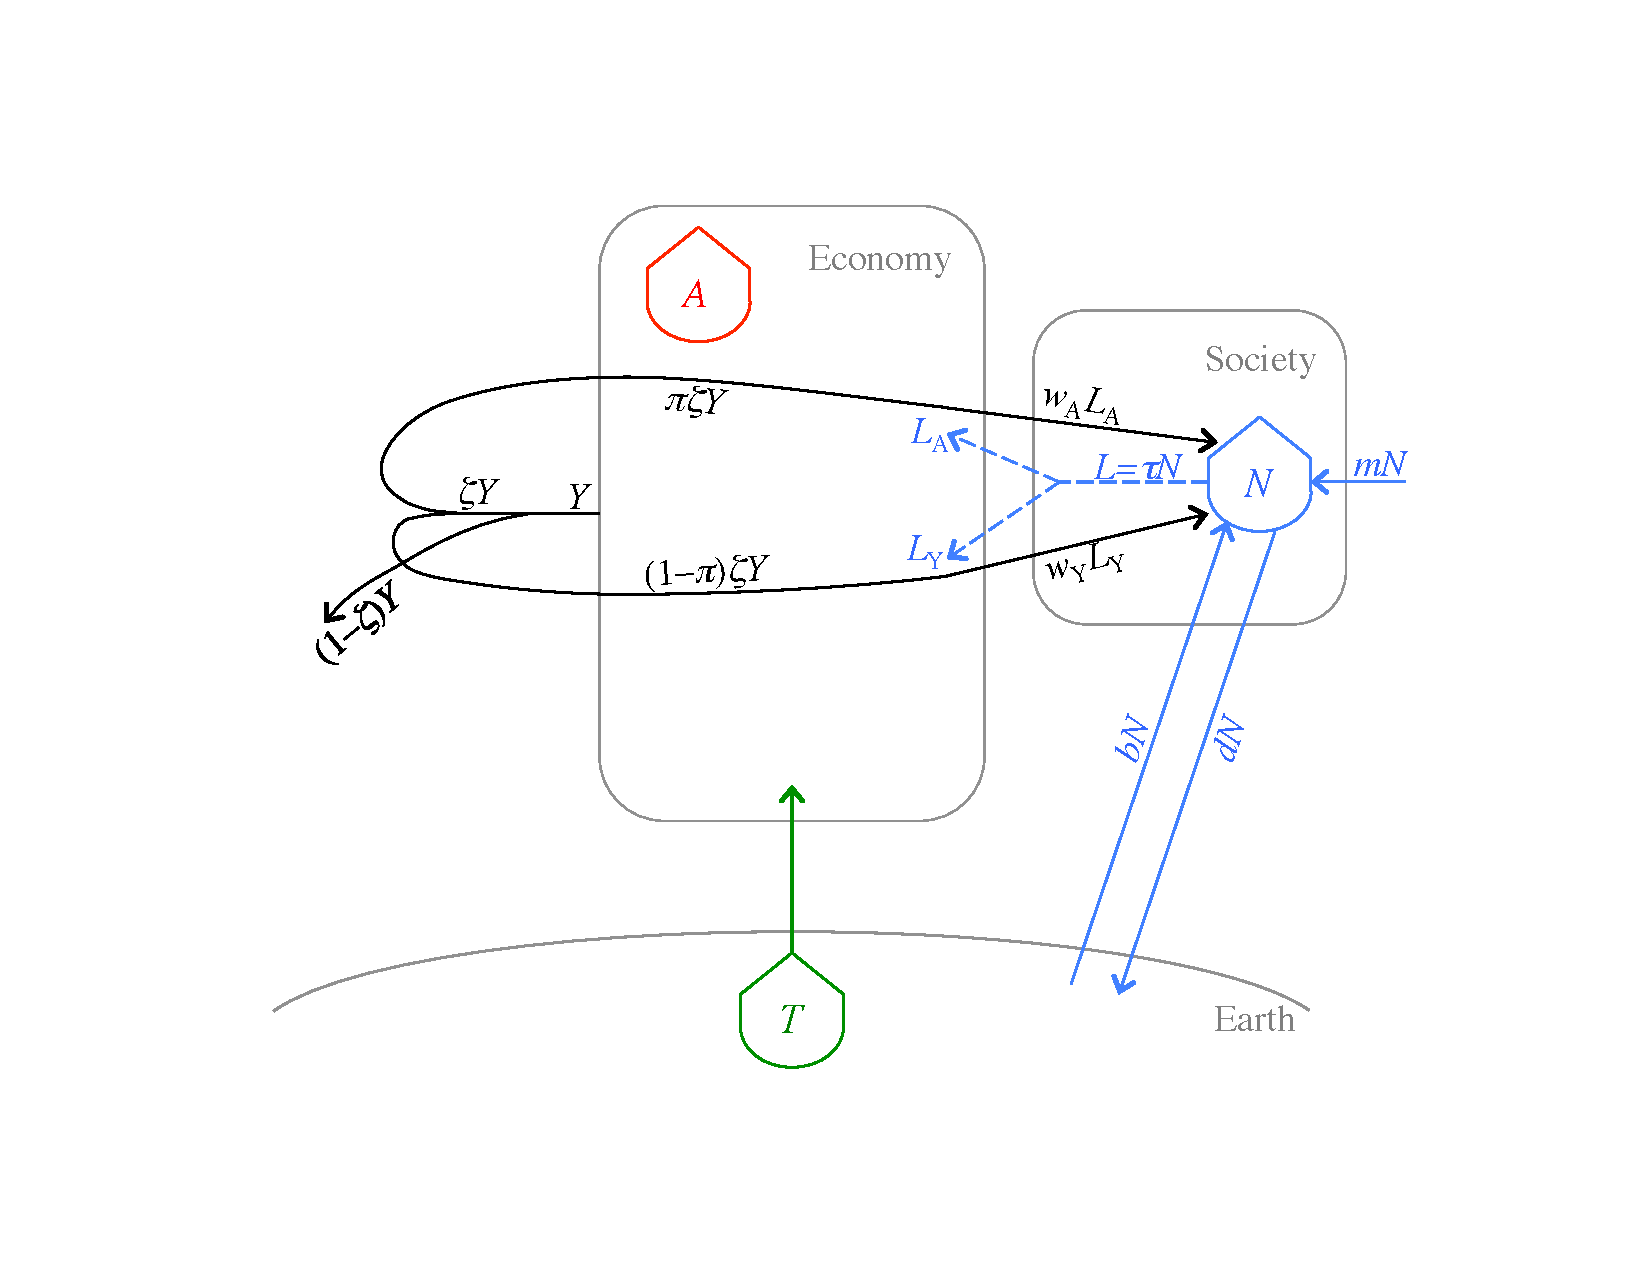
\includegraphics[width=\textwidth]{figure_other/ModelWithoutEnergy.pdf}
    \caption{Dynamic model without energy.}
  \end{center}
\end{figure}

For \citet{Jones:2001wn}, economic production ($y$) is given by

\begin{equation} \label{eq:Jones_production_function}
	y_\mathrm{t} = a_\mathrm{t} ^\sigma l_\mathrm{Y,t} ^\beta t_\mathrm{t} ^{1-\beta} \epsilon_\mathrm{t}
\end{equation}

\noindent where $a_\mathrm{t}$ is the indexed stock of ideas, $l_\mathrm{Y,t}$ is indexed labor in the goods producing sector, $t_\mathrm{t}$ is indexed land (always 1.0), and $\varepsilon_\mathrm{t}$ is an exogenous shock parameter. The subscript ``t'' indicates time (measured in years). Any symbol in a equation with subscript ``$\mathrm{t}$'' indicates a time-varying quantity. Symbols without subscript ``$\mathrm{t}$'' indicate time-invariant quantities. Lowercase variable names represent unitless, indexed quantities. The indexed factors of production ($a_\mathrm{t}$, $l_\mathrm{t}$, and $t_\mathrm{t}$) are defined relative to a base year ($\mathrm{t} = 0$):

\begin{equation} \label{eq:index_y}
	y_\mathrm{t} \equiv \frac{Y_\mathrm{t}}{Y_\mathrm{0}}
\end{equation}

\begin{equation} \label{eq:index_a}
	a_\mathrm{t} \equiv \frac{A_\mathrm{t}}{A_\mathrm{0}}
\end{equation}

\begin{equation} \label{eq:index_l}
	l_\mathrm{Y,t} \equiv \frac{L_\mathrm{Y,t}}{L_\mathrm{Y,0}}
\end{equation}

\begin{equation} \label{eq:index_t}
	t_\mathrm{t} \equiv \frac{T_\mathrm{t}}{T_\mathrm{0}} = 1.0
\end{equation}

\noindent with $Y_\mathrm{t}$ representing economic output (in 2005\$/year), $A_\mathrm{t}$ representing the stock of knowledge (in units of ideas), $L_\mathrm{Y,t}$ representing labor in the production sector (in workers/year), and $T_\mathrm{t}$ representing the stock of available land (in m$^2$).

Our model for preferences between consumption and childrearing is based on the utility function from \citet{Jones:2001wn}:

\begin{equation} \label{eq:utility_function}
	u_\mathrm{t}(c_\mathrm{t}, b_\mathrm{t}) = u_\mathrm{c,t} + u_\mathrm{b,t} = \frac{1-\mu}{1-\gamma} \left(\frac{k_\mathrm{c} \tilde c_\mathrm{t}}{U_\mathrm{c,0}} \right)^{1-\gamma} + \frac{\mu}{1-\eta} \left(\frac{k_\mathrm{b} \tilde b_\mathrm{t}}{U_\mathrm{b,0}} \right)^{1-\eta}
\end{equation}

\noindent where $\mu$, $\gamma$, and $\eta$ are dimensionless parameters with values between 0 and 1; $k_\mathrm{c}$ and $k_\mathrm{b}$ represent the utility obtained per unit consumption or birth (in units of utils/\$ and utils/birth, respectively); and $U_{\mathrm{c,0}}$ and $U_{\mathrm{b,0}}$ are the utility derived from consumption and childrearing, respectively, at $\mathrm{t} = 0$ (in units of utils/year). $\tilde c_\mathrm{t}$ is the rate of the individual's consumption in 2005\$/year-capita and $\tilde b_\mathrm{t}$ is the rate of births in births/year-capita. $u_\mathrm{c,t}$ and $u_\mathrm{b,t}$ represent utility obtained from consumption and births, represented by the first and second terms, respectively, on the right side of Equation~\ref{eq:utility_function}. $\tilde c_\mathrm{t}$ represents the rate of consumption above subsistence level ($\bar c$ in 2005\$/year-capita), and $\tilde b_\mathrm{t}$ represents the rate of births above some long-run birth rate ($\bar b$, in births/year-capita).

\begin{equation} \label{eq:c_tilde}
	\tilde c_\mathrm{t} \equiv c_\mathrm{t} - \bar c
\end{equation}

\begin{equation} \label{eq:b_tilde}
	\tilde b_\mathrm{t} \equiv b_\mathrm{t} - \bar b
\end{equation}

The first order condition on the utility function (Equation \ref{eq:utility_function}) requires that a person will obtain equal incremental utility from spending additional time consuming or rearing children:

\begin{equation} \label{eq:first_order_condition_def}
	\frac{\partial u_{c,t}}{\partial \tau_\mathrm{t}} = \frac{\partial u_{b,t}}{\partial \tau_\mathrm{t}}
\end{equation}

\noindent where $\tau_\mathrm{t} \in (0,1)$. $\tau_\mathrm{t}$ can be interpreted on a per-person basis as worked hours per total available working time. Or, if each individual in the population is assumed to be either a worker or a childrearer, $\tau_\mathrm{t}$ represents the ratio of workers to total population ($L_\mathrm{t}/N_\mathrm{t}$). The first order condition simplifies to 

\begin{equation} \label{eq:first_order_condition_simplified}
	\frac{\partial u_\mathrm{t}/ \partial\tilde b_\mathrm{t}}{\partial u_\mathrm{t}/ \partial\tilde c_\mathrm{t}} = \frac{w_\mathrm{t}}{\nu},
\end{equation}

\noindent where $w_\mathrm{t}$ is the wage rate (in 2005\$/year-worker) and $\nu$ is a birth efficiency (in births/year-capita). $w_\mathrm{t}$ and $\nu$ appear in Equations \ref{eq:consumption_constraint} and \ref{eq:birth_constraint}, given by:

\begin{equation}\label{eq:pop_work}
	L_\mathrm{t} = \tau_\mathrm{t} N_\mathrm{t}
\end{equation}

\begin{equation} \label{eq:consumption_constraint}
	c_\mathrm{t} = w_\mathrm{t} \tau_\mathrm{t}
\end{equation}

\begin{equation} \label{eq:birth_constraint}
	b_\mathrm{t} = \nu (1-\tau_\mathrm{t})
\end{equation}

\noindent $N_\mathrm{t}$ is the total population (in persons), and $L_\mathrm{t}$ is the total amount of available labor in the economy (in workers/year). So, $(1-\tau_\mathrm{t})$ represents the fraction of available time spent on childrearing (unitless or time childrearing per total time). It is worth noting that the units of $\tau_\mathrm{t}$ can also be defined in terms of workers/capita, as shown in Equation~\ref{eq:pop_work}.

Applying the first order condition (Equation \ref{eq:first_order_condition_simplified}) with Equations \ref{eq:consumption_constraint} and \ref{eq:birth_constraint} yields an equation that describes preferences for consumption and childrearing:

\begin{equation} \label{eq:FOC_and_time_constraints}
	\frac{1}{\nu \mu} \frac{U_\mathrm{b,0}}{k_\mathrm{b}} \left( \frac{k_\mathrm{b}}{U_\mathrm{b,0}} \tilde b_\mathrm{t} \right) ^{\eta} 
	= \frac{1}{w_\mathrm{t}(1-\mu)} \frac{U_\mathrm{c,0}}{k_\mathrm{c}}  \left( \frac{k_\mathrm{c}}{U_\mathrm{c,0}} \tilde c_\mathrm{t} \right)^\gamma .
\end{equation}

\noindent where $\gamma$, $\eta$, and $\mu$ are constants; $k_\mathrm{b}$ and $k_\mathrm{c}$ represent the utility per unit birth and utility per unit of consumption; and $U_\mathrm{b,0}$ and $U_\mathrm{c,0}$ are the total utilities derived from births and consumption respectively in the first year of the simulation. Since $U_\mathrm{b,0}$, $U_\mathrm{c,0}$, $k_\mathrm{b}$, $k_\mathrm{c}$, and $\mu$ are all constants that can be moved to the front of either side of the equation, we grouped these parameters together into a new parameter called $G$.

\begin{equation} \label{eq:FOC_with_G}
 	\tilde b_\mathrm{t}^\eta = \frac{\tilde c_\mathrm{t}^\gamma}{w_\mathrm{t}} G
\end{equation}

\noindent where $G$ is also constant over time.

Labor is split between two sectors; one devoted to innovation and producing new ideas ($A_\mathrm{t}$) and the other devoted to producing goods ($Y_\mathrm{t}$). The split between these sectors can be expressed in terms of the wages paid to workers in each sector as shown in the equations below:

\begin{equation} \label{eq:knowledge_comp}
	w_\mathrm{A,t} L_\mathrm{A,t} = \pi \zeta Y_\mathrm{t}
\end{equation}

\begin{equation} \label{eq:labor_comp}
	w_\mathrm{Y,t} L_\mathrm{Y,t} = (1-\pi) \zeta Y_\mathrm{t}
\end{equation}

\noindent where $w_\mathrm{A,t}$ and $w_\mathrm{Y,t}$ are the wages paid to workers in the knowledge and goods producing sectors respectively (in 2005\$/year-worker), and $L_\mathrm{A,t}$ and $L_\mathrm{Y,t}$ represent the number of workers employed in each of the sectors (in workers/year). $\zeta$ represents the fraction of economic output ($Y_\mathrm{t}$) that goes toward wages. The dimensionless variable $\pi$ is the fraction of the economy's total output ($Y_\mathrm{t}$) that is devoted to compensating inventors in the knowledge sector. The total labor supply ($L_\mathrm{t}$) is constrained as the sum of the labor supply in the two sectors.

\begin{equation} \label{eq:labor_supply}
	L_\mathrm{t} = L_\mathrm{A,t} + L_\mathrm{Y,t}
\end{equation}

The two labor supplies can be expressed as indexed quantities when convenient.

\begin{equation}
	l_\mathrm{Y,t} \equiv \frac{L_\mathrm{Y,t}}{L_\mathrm{Y,0}}
\end{equation}

\begin{equation}
	l_\mathrm{A,t} \equiv \frac{L_\mathrm{A,t}}{L_\mathrm{A,0}}
\end{equation}

In equilibrium, it is expected that wages paid to workers in each sector will be equal.

\begin{equation} \label{eq:wage_equality}
	w_\mathrm{A,t} = w_\mathrm{Y,t} = w_\mathrm{t}
\end{equation}

Wage equality (Equation~\ref{eq:wage_equality}) allows $\pi_\mathrm{t}$ to be directly proportional to the fraction of the total employed population working in the knowledge sector in static equilibrium.

\begin{equation} \label{eq:pi}
	\pi = \frac{L_\mathrm{A,t}}{L_\mathrm{t}}
\end{equation}

Two differential equations describe the growth of knowledge ($A_\mathrm{t}$) and population ($N_\mathrm{t}$) over time. The rate of change in the indexed stock of knowledge ($a_\mathrm{t}$) is given by

\begin{equation} \label{eq:da_dt}
	\frac{\mathrm{d}a_\mathrm{t}}{\mathrm{d}t} = \delta' l_\mathrm{A,t}^\lambda a_\mathrm{t}^\phi
\end{equation}

\noindent where $\lambda$, and $\phi$ are constants, and $l_\mathrm{A,t}$ is the indexed labor in the knowledge sector of the economy. $\delta'$ is given by,

\begin{equation} \label{eq:delta}
	\delta' = \delta L_\mathrm{A,0}^\lambda A_\mathrm{0}^{(\phi - 1)}
\end{equation}

\noindent where $\delta$ is a constant and $L_\mathrm{A,0}$ and $A_\mathrm{0}$ represent the labor in the knowledge sector and stock of knowledge in the first year of the simulation. 

The rate of change of indexed population ($n$) is a function of birth and mortality rates ($b_\mathrm{t}$ and $d_\mathrm{t}$ in births/year-capita and deaths/year-capita, respectively):

\begin{equation} \label{eq:dn_dt}
	\frac{\mathrm{d}n_\mathrm{t}}{\mathrm{d}t} = (b_\mathrm{t} - d_\mathrm{t} + m) n_\mathrm{t},
\end{equation}

\noindent where $b_\mathrm{t}$ is the birth rate from Equation~\ref{eq:utility_function}, $n_\mathrm{t}$ is the indexed population, $d_\mathrm{t}$ is the mortality rate in deaths/year-capita, and $m$ is the average rate of net migration in the United States. The form of the mortality equation is taken from \citet{Jones:2001wn} as

\begin{equation} \label{eq:mortality_rate}
	d_\mathrm{t} = \frac{1}{\omega_\mathrm{1} z_\mathrm{t}^{\omega_\mathrm{2}} + \omega_\mathrm{3} z_\mathrm{t}} + \bar d,
\end{equation}

\noindent where $d_\mathrm{t}$ is the mortality rate and $\bar d$ is the long-run mortality rate **** Caleb: what is the value of $\bar{d}$? ****, both in units of deaths/year-capita. $\omega_\mathrm{1}$, $\omega_\mathrm{2}$, and $\omega_\mathrm{3}$ are fitted parameters. The ratio of consumption to the subsistence level is given by $z_\mathrm{t}$:

\begin{equation} \label{eq:z}
	z_\mathrm{t} = \frac{c_\mathrm{t}}{\bar c} - 1
\end{equation}

\noindent which is an indicator of the mortality rate through Equation~\ref{eq:mortality_rate}.

%++++++++++++++++++++++++++++++
\subsection{Tuning: basic model}
\label{sec:basic_model_tuning}
%++++++++++++++++++++++++++++++

To tune the basic model to match U.S. historical data from 1980--2011, we estimate values for the fitting parameters, including $\beta$ and $\sigma$ from Equation~\ref{eq:Jones_production_function}; $\bar c$ and $\bar b$ from Equations \ref{eq:c_tilde} and \ref{eq:b_tilde}, respectively; $\tau_\mathrm{t}$ for all years based on year 1980 ($\tau_\mathrm{1980} = L_\mathrm{A,1980}/L_\mathrm{1980}$); $\mu$, $\nu$, and $G$ from Equation~\ref{eq:FOC_with_G}; $\zeta$ from Equation~\ref{eq:knowledge_comp}; $\pi$ from Equation \ref{eq:pi}; $\lambda$ and $\phi$ from Equation \ref{eq:da_dt}; $\delta$ and $A_\mathrm{0}$ from Equation \ref{eq:delta}; $m$ from Equation \ref{eq:dn_dt}; and $\omega_1$, $\omega_2$, $\omega_3$, and $\bar d$ from Equation \ref{eq:mortality_rate}. We tuned the basic model with least-squares optimization by comparing outputs of the model ($y_\mathrm{t}$, $w_\mathrm{t}$, $c_\mathrm{t}$, $\tau_\mathrm{t}$, $l_\mathrm{Y,t}$, $l_\mathrm{A,t}$, $n_\mathrm{t}$, $b_{\mathrm{t}}$, and $d_\mathrm{t}$) to historical data. The following subsections discuss historical data, development of ``ground truth'' time series, and the parameter estimation process.

%------------------------------
\subsubsection{Historical data}
\label{sec:basic_model_historical_data}
%------------------------------

We collected historical time series data for United States on economic output ($Y_\mathrm{t}$), total labor force ($L_\mathrm{t}$), knowledge sector labor force ($L_\mathrm{A,t}$), population ($N_\mathrm{t}$), births ($B_\mathrm{t}$), deaths ($D_\mathrm{t}$), and wages ($w_\mathrm{t}$). Historical data was obtained for the years 1980--2011 unless otherwise noted. 

We measure economic output ($Y_\mathrm{t}$) by gross domestic product (GDP). We obtained GDP data, in real 2005 U.S. dollars per year, from the World Bank's Global Economic Prospects (GEP) database \citep{WorldBankGEP:2013a}.

We obtained total labor force data ($L_\mathrm{t}$) from the United States Bureau of Labor Statistics (BLS) in units of total number of employed persons \citep{BLS:2013a}. 

We quantify the size of the knowledge sector labor force ($L_\mathrm{A,t}$) by the total number of researchers, where researchers, i.e., people working in research and development (R\&D) positions in STEM (science, technology, engineering, mathematics) fields. (Note that \citet{Jones:2001wn} does not provide a specific definition of knowledge sector labor.) Data on the knowledge sector labor force was obtained from the Organisation of Economic Co-operation and Development (OECD) time series on research and development R\&D personel \citep{OECDStatExtracts:2013a}. Data are available from 1981--2007, with odd years only between 1985 and 1999, so we extrapolated linearly forward from 2007 to 2011 and backward from 1981 to 1980. We interpolated linearly for even years between 1985 and 1999.

We define population ($N_\mathrm{t}$) as the total number of people living in the U.S. each year. We obtained population data from the World Bank's World Development Indicators (WDI) database \citep{WorldBankWDI:2013a}.

We define births ($B_\mathrm{t}$) as the number of births within the U.S. each year. We acquired data on the number of births from the Center for Diesease Control (CDC) time series on births in the U.S. \citep{Martin:2012tc, Hamilton:2012ww}

We define deaths ($D_\mathrm{t}$) as the number of deaths within the U.S. each year. We acquired data on the number of deaths from the Center for Diesease Control (CDC) time series on deaths in the U.S. \citep{Murphy:2013vg, Hoyert:2012tv}.

We define wages ($w_\mathrm{t}$) as the yearly salarly that is earned by someone working in either the knowledge or manufacturing sector (because the wages will be equivalent in dynamic equilibrium, by Equation~\ref{eq:wage_equality}). Wage data was obtained from the U.S. Census Bureau's annual population survey **** Caleb: need reference ****, which contains data on average per capita income in the U.S.

**** Heun: create graph of historical historical data. Perhaps a Lattice plot of some type? ****

%------------------------------
\subsubsection{``Ground truth'' information}
\label{sec:basic_model_ground_truth}
%------------------------------

Based on the historical data outlined above, we calculated ``historical'' time series for other important parameters in the model. To obtain $b_\mathrm{t}$ in units of births/year-person, we divided the CDC birth data ($B_\mathrm{t}$) by the total population ($N_\mathrm{t}$) for each year. To obtain $d_\mathrm{t}$ in units of deaths/year-person, we divided the CDC mortality data ($D_\mathrm{t}$) by the total population ($N_\mathrm{t}$) for each year.

Per capita income data were multiplied by the total population and then divided by the labor force to obtain a wage time series ($w_\mathrm{t}$) in 2005\$/year-worker. Using Equation \ref{eq:pop_work}, we calculated historical values for $\tau_\mathrm{t}$. Using the historical $\tau_\mathrm{t}$ values and Equation \ref{eq:consumption_constraint} we were able to calculate historical values of consumption ($c_\mathrm{t}$). 

We used 1980 values of $\tau_\mathrm{t}$ and $b_\mathrm{t}$ to calculate a value for $\nu$ **** Heun: give the value of $\nu$ here **** that we hold constant through time. We used 1980 values for $L_\mathrm{A,1980}$ and $L_{1980}$ to calculate an invariant value for $\pi_\mathrm{t}$. **** Caleb: Is $\pi$ really invariant through the simulation? If so, we need to remove the subscript ``t'' everywhere. **** **** Heun: Give the value of $\pi$ or $\pi_\mathrm{t}$ here. ****

To determine values of the three mortality function fitting parameters ($\omega_\mathrm{1}$, $\omega_\mathrm{2}$, and $\omega_\mathrm{3}$), we used a least-squares minimization. Historical values of $z_\mathrm{t}$ were calculated from Equation \ref{eq:z} by using the calculated historical values of consumption ($c_\mathrm{t}$). These historical $z_\mathrm{t}$ values were used to calculated a predicted $d_\mathrm{t}$ value that was then compared to the historical $d_\mathrm{t}$ values for the minimzation. 

To determine $\eta$ and $\gamma$

**** Heun: show graph here ****

%------------------------------
\subsubsection{Parameter estimation}
\label{sec:basic_model_parameter_estimation}
%------------------------------

**** Heun: Create a table of the estimated parameters. ****




%++++++++++++++++++++++++++++++
\subsection{Results: basic model}
\label{sec:Results_basic_model}
%++++++++++++++++++++++++++++++

**** Heun: develop graphs and other results based on Caleb's work with the basic model. ****


%%%%%%%%%%%%%%%%%%%%%%%%%%%%%%%%
\section{Enhanced model (with energy and capital stock)}
\label{sec:Enhanced_model}
%%%%%%%%%%%%%%%%%%%%%%%%%%%%%%%%

%++++++++++++++++++++++++++++++
\subsection{Enhanced model development}
\label{sec:enhanced_model_development}
%++++++++++++++++++++++++++++++

We now enhance the basic model with both energy flows and capital stock.

\begin{figure} \label{fig:ModelWithEnergy}
  \begin{center}
    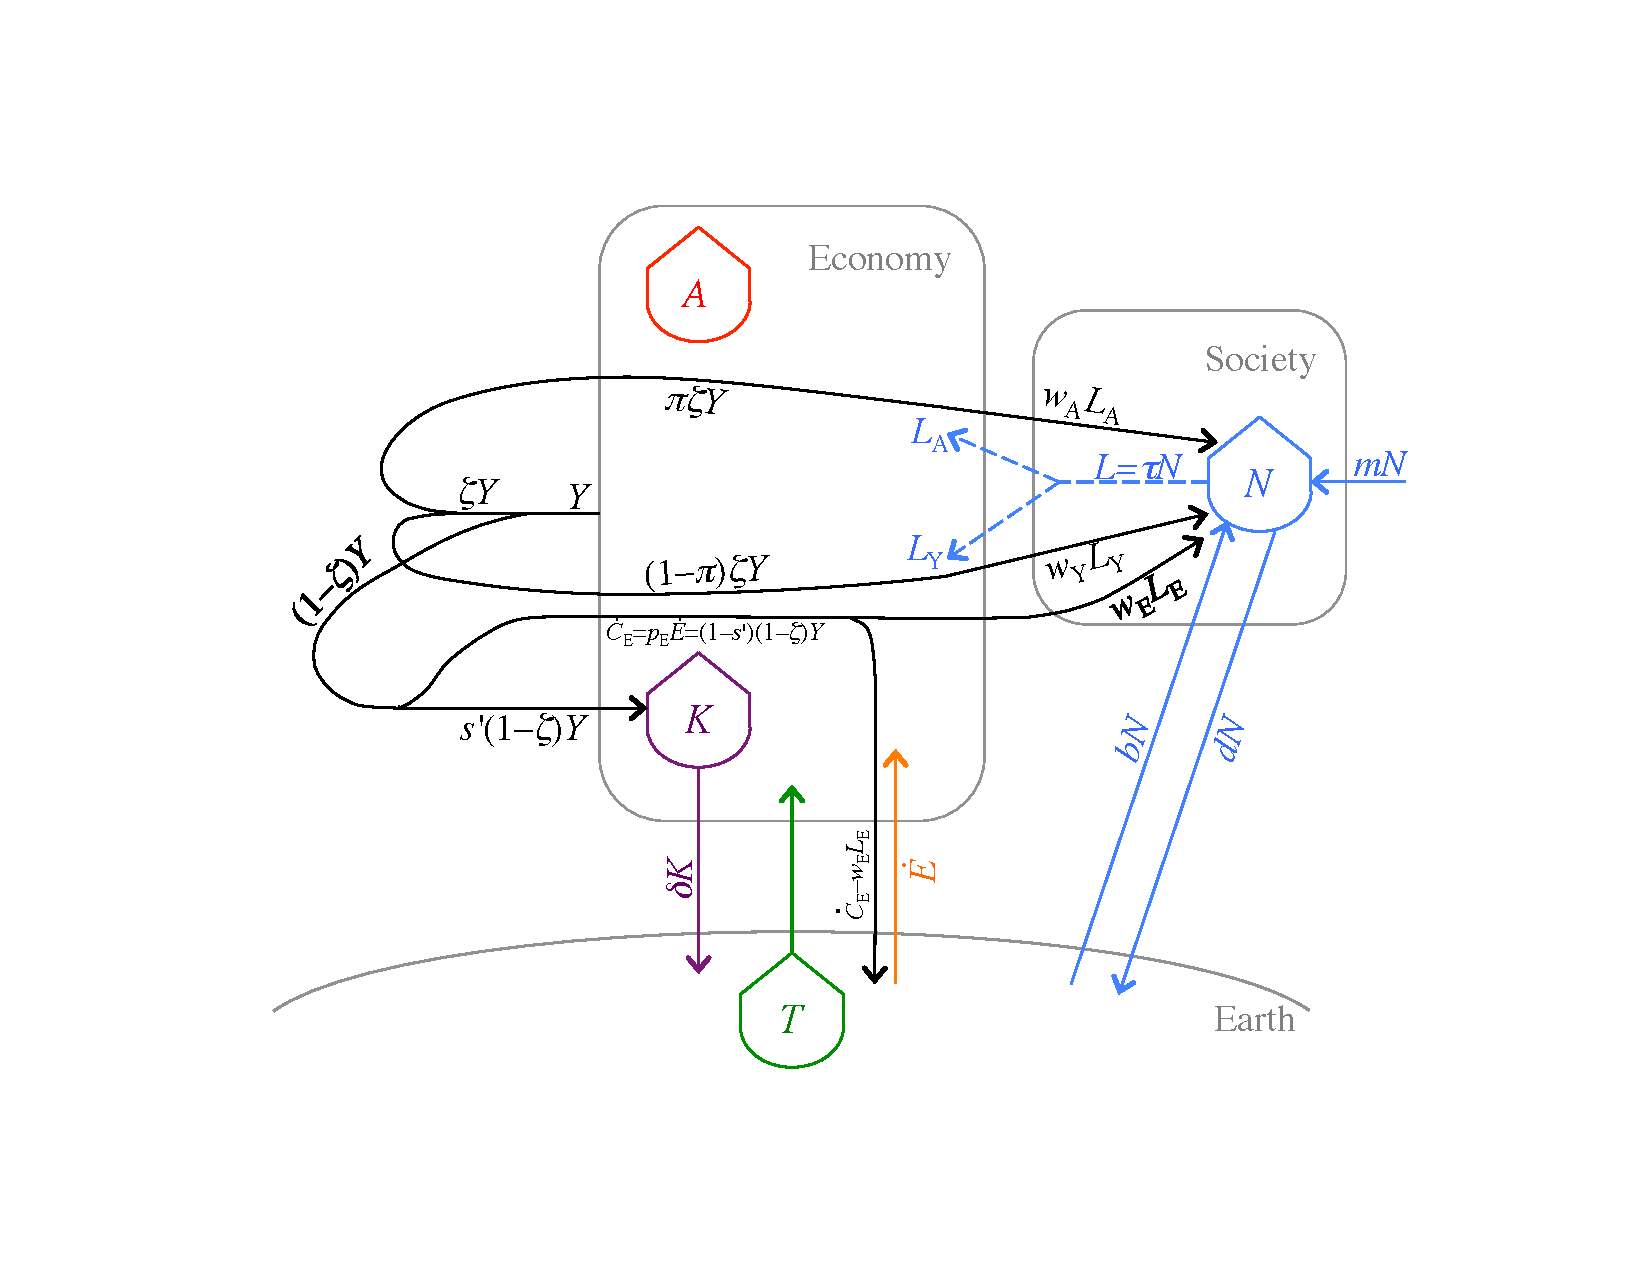
\includegraphics[width=\textwidth]{figure_other/ModelWithEnergy.pdf}
    \caption{Dynamic model with energy.}
  \end{center}
\end{figure}

%++++++++++++++++++++++++++++++
\subsection{Tuning: enhanced model}
\label{sec:enhanced_model_tuning}
%++++++++++++++++++++++++++++++

**** Caleb: discuss the process you used to tune the enhanced model. ****

%------------------------------
\subsubsection{Historical data}
\label{sec:enhanced_model_historical_data}
%------------------------------

%------------------------------
\subsubsection{``Ground truth'' information}
\label{sec:enhanced_model_ground_truth}
%------------------------------

%------------------------------
\subsubsection{Parameter estimation}
\label{sec:enhanced_model_parameter_estimation}
%------------------------------


%++++++++++++++++++++++++++++++
\subsection{Results: enhanced model}
\label{sec:enhanced_model_results}
%++++++++++++++++++++++++++++++

**** MKH to develop graphs and other results based on Caleb's existing work ****


%%%%%%%%%%%%%%%%%%%%%%%%%%%%%%%
\section{Implications}
\label{sec:Implications}
%%%%%%%%%%%%%%%%%%%%%%%%%%%%%%%


%%%%%%%%%%%%%%%%%%%%%%%%%%%%%%%
\section{Conclusion}
\label{sec:Conclustion}
%%%%%%%%%%%%%%%%%%%%%%%%%%%%%%%


%%%%%%%%%%%%%%%%%%%%%%%%%%%%%%%
\section*{Acknowledgements}
\label{sec:Acknowledgements}
%%%%%%%%%%%%%%%%%%%%%%%%%%%%%%%

**** Comment before submission **** Funding for Caleb Reese was provided by the Integrated Science Research Institute at Calvin College. Partial funding for Matthew Kuperus Heun was provided by a Calvin College Research Fellowship. 

%%%%%%%%%%%%%%%%%%%%%%%%%%%%%%%
\section*{Reproducible Research}
%%%%%%%%%%%%%%%%%%%%%%%%%%%%%%%

**** Comment before submission **** In the spirit of Reproducible Research \citep{Gandrud:2013vx}, all data, spreadsheets, \texttt{R} code \citep{R}, \texttt{EES} code \citep{EES}, and other materials associated with this paper can be found at\\*
\protect\url{https://github.com/MatthewHeun/EconDynamicLongwaveModel}.



%%%%%%%%%%%%%%%%%%%%%%%%%%%%%%%
%% Bibliography (via BibTeX)
%%%%%%%%%%%%%%%%%%%%%%%%%%%%%%%
\bibliographystyle{DeGruyter}
\bibliography{ReeseHeunJournalPaper}

\end{document}